\documentclass[8pt,aspectratio=169]{beamer}
\usetheme{Madrid}
\usepackage{graphicx}
\usepackage{booktabs}
\usepackage{adjustbox}
\usepackage{multicol}
\usepackage{amsmath}
\usepackage{amssymb}
\usepackage{listings}
\usepackage{xcolor}

% Color definitions
\definecolor{mlblue}{RGB}{0,102,204}
\definecolor{mlpurple}{RGB}{51,51,178}
\definecolor{mllavender}{RGB}{173,173,224}
\definecolor{mllavender2}{RGB}{193,193,232}
\definecolor{mllavender3}{RGB}{204,204,235}
\definecolor{mllavender4}{RGB}{214,214,239}
\definecolor{mlorange}{RGB}{255, 127, 14}
\definecolor{mlgreen}{RGB}{44, 160, 44}
\definecolor{mlred}{RGB}{214, 39, 40}
\definecolor{mlgray}{RGB}{127, 127, 127}

% Additional colors for template compatibility
\definecolor{lightgray}{RGB}{240, 240, 240}
\definecolor{midgray}{RGB}{180, 180, 180}

% Solidity colors
\definecolor{solkeyword}{RGB}{0,102,153}
\definecolor{solstring}{RGB}{163,21,21}
\definecolor{solcomment}{RGB}{0,128,0}
\definecolor{solnumber}{RGB}{0,128,128}

% Solidity language definition
\lstdefinelanguage{Solidity}{
  keywords={pragma, solidity, contract, function, public, private, external, internal, view, pure, payable, returns, return, if, else, for, while, mapping, address, uint, uint256, int, string, bool, bytes, bytes32, event, emit, modifier, require, constructor, memory, storage, calldata, msg, sender, value, this, new, delete, true, false},
  keywordstyle=\color{solkeyword}\bfseries,
  sensitive=true,
  comment=[l]{//},
  morecomment=[s]{/*}{*/},
  commentstyle=\color{solcomment}\ttfamily,
  stringstyle=\color{solstring}\ttfamily,
  morestring=[b]',
  morestring=[b]"
}

% Apply custom colors to Madrid theme
\setbeamercolor{palette primary}{bg=mllavender3,fg=mlpurple}
\setbeamercolor{palette secondary}{bg=mllavender2,fg=mlpurple}
\setbeamercolor{palette tertiary}{bg=mllavender,fg=white}
\setbeamercolor{palette quaternary}{bg=mlpurple,fg=white}
\setbeamercolor{structure}{fg=mlpurple}
\setbeamercolor{section in toc}{fg=mlpurple}
\setbeamercolor{subsection in toc}{fg=mlblue}
\setbeamercolor{title}{fg=mlpurple}
\setbeamercolor{frametitle}{fg=mlpurple,bg=mllavender3}
\setbeamercolor{block title}{bg=mllavender2,fg=mlpurple}
\setbeamercolor{block body}{bg=mllavender4,fg=black}

\setbeamertemplate{navigation symbols}{}
\setbeamertemplate{itemize items}[circle]
\setbeamertemplate{enumerate items}[default]
\setbeamersize{text margin left=5mm,text margin right=5mm}

\newcommand{\bottomnote}[1]{%
\vfill
\vspace{-2mm}
\textcolor{mllavender2}{\rule{\textwidth}{0.4pt}}
\vspace{1mm}
\footnotesize
\textbf{#1}
}

% TikZ and pgfplots packages
\usepackage{tikz}
\usepackage{pgfplots}
\pgfplotsset{compat=1.18}
\usetikzlibrary{arrows.meta, positioning, shapes.geometric, shapes.symbols, calc, decorations.pathmorphing, mindmap}

\title{Layer 2 Scaling Solutions: A Visual Introduction}
\subtitle{Standalone Mini-Lecture}
\author{Prof.~Dr.~Joerg Osterrieder}
\institute{University Lecture Series}
\date{\today}
\begin{document}

% Frame 1: Title
\begin{frame}[plain]
\vspace{2cm}
\begin{center}
{\Huge\color{mlpurple} Layer 2 Scaling Solutions: A Visual Introduction}\\[0.4cm]
{\Large\color{mlblue} Standalone Mini-Lecture}\\[0.3cm]
\textcolor{mlgray}{\rule{6cm}{0.4pt}}\\[0.3cm]
{\small\itshape ``Rollups are the only trustless scaling solution for Ethereum'' -- Vitalik Buterin}\\[1.5cm]
{\normalsize Prof.~Dr.~Joerg Osterrieder}\\[0.2cm]
{\small University Lecture Series}\\[0.2cm]
{\small \today}
\end{center}

\bottomnote{This mini-lecture covers Layer 2 scaling: the blockchain trilemma, rollup types, how rollups work, bridge risks, and the current L2 ecosystem.}
\end{frame}

% Frame 2: The Scaling Problem
\begin{frame}{The Scaling Problem}
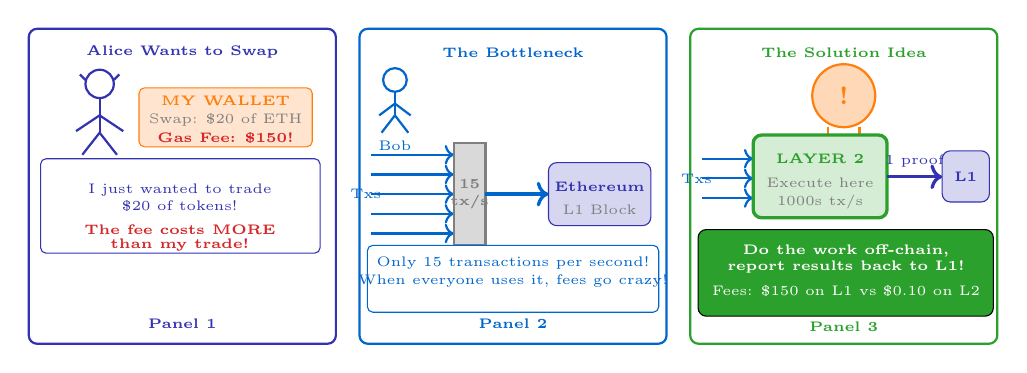
\begin{tikzpicture}
  % Panel borders
  \draw[thick, mlpurple, rounded corners=3pt] (0.1,0.2) rectangle (4.0,4.2);
  \draw[thick, mlblue,   rounded corners=3pt] (4.3,0.2) rectangle (8.2,4.2);
  \draw[thick, mlgreen,  rounded corners=3pt] (8.5,0.2) rectangle (12.4,4.2);

  % --- Panel 1: Alice shocked by gas fees ---
  \node[font=\tiny\bfseries, mlpurple] at (2.05,3.9) {Alice Wants to Swap};
  % Alice stick figure
  \draw[mlpurple,thick] (1.0,3.5) circle (0.18);
  \draw[mlpurple,thick] (1.0,3.32) -- (1.0,2.88);
  \draw[mlpurple,thick] (1.0,3.1) -- (0.7,2.9);
  \draw[mlpurple,thick] (1.0,3.1) -- (1.3,2.9);
  \draw[mlpurple,thick] (1.0,2.88) -- (0.78,2.60);
  \draw[mlpurple,thick] (1.0,2.88) -- (1.22,2.60);
  \node[font=\tiny, mlpurple] at (1.0,2.45) {Alice};
  % Shocked expression lines
  \draw[mlpurple,thick] (0.82,3.55) -- (0.75,3.62);
  \draw[mlpurple,thick] (1.18,3.55) -- (1.25,3.62);
  % Wallet box
  \draw[fill=mlorange!20, draw=mlorange, rounded corners=2pt] (1.5,2.7) rectangle (3.7,3.45);
  \node[font=\tiny\bfseries, mlorange, align=center] at (2.6,3.28) {MY WALLET};
  \node[font=\tiny, mlgray, align=center] at (2.6,3.05) {Swap: \$20 of ETH};
  \node[font=\tiny\bfseries, mlred, align=center] at (2.6,2.82) {Gas Fee: \$150!};
  % Speech bubble
  \draw[fill=white, draw=mlpurple, rounded corners=2pt] (0.25,1.35) rectangle (3.8,2.55);
  \node[font=\tiny, mlpurple, align=center] at (2.02,2.15) {I just wanted to trade};
  \node[font=\tiny, mlpurple, align=center] at (2.02,1.95) {\$20 of tokens!};
  \node[font=\tiny\bfseries, mlred, align=center] at (2.02,1.65) {The fee costs MORE};
  \node[font=\tiny\bfseries, mlred, align=center] at (2.02,1.45) {than my trade!};
  \node[font=\tiny\bfseries, mlpurple] at (2.05,0.45) {Panel 1};

  % --- Panel 2: Bottleneck explanation ---
  \node[font=\tiny\bfseries, mlblue] at (6.25,3.9) {The Bottleneck};
  % Bob stick figure
  \draw[mlblue,thick] (4.75,3.55) circle (0.15);
  \draw[mlblue,thick] (4.75,3.4) -- (4.75,3.1);
  \draw[mlblue,thick] (4.75,3.25) -- (4.55,3.1);
  \draw[mlblue,thick] (4.75,3.25) -- (4.95,3.1);
  \draw[mlblue,thick] (4.75,3.1) -- (4.58,2.88);
  \draw[mlblue,thick] (4.75,3.1) -- (4.92,2.88);
  \node[font=\tiny, mlblue] at (4.75,2.72) {Bob};
  % Many tx arrows on left
  \draw[->, thick, mlblue] (4.45,2.6) -- (5.5,2.6);
  \draw[->, thick, mlblue] (4.45,2.35) -- (5.5,2.35);
  \draw[->, thick, mlblue] (4.45,2.1) -- (5.5,2.1);
  \draw[->, thick, mlblue] (4.45,1.85) -- (5.5,1.85);
  \draw[->, thick, mlblue] (4.45,1.6) -- (5.5,1.6);
  \node[font=\tiny, mlblue, align=center] at (4.38,2.1) {Txs};
  % Narrow pipe (bottleneck)
  \draw[fill=mlgray!30, draw=mlgray, thick] (5.5,1.45) rectangle (5.9,2.75);
  \node[font=\tiny\bfseries, mlgray, align=center] at (5.7,2.1) {15\\tx/s};
  % Single arrow out
  \draw[->, very thick, mlblue] (5.9,2.1) -- (6.7,2.1);
  % Ethereum box
  \draw[fill=mlpurple!20, draw=mlpurple, rounded corners=3pt] (6.7,1.7) rectangle (8.0,2.5);
  \node[font=\tiny\bfseries, mlpurple, align=center] at (7.35,2.2) {Ethereum};
  \node[font=\tiny, mlgray, align=center] at (7.35,1.9) {L1 Block};
  % Speech bubble
  \draw[fill=white, draw=mlblue, rounded corners=2pt] (4.4,0.6) rectangle (8.1,1.45);
  \node[font=\tiny, mlblue, align=center] at (6.25,1.22) {Only 15 transactions per second!};
  \node[font=\tiny, mlblue, align=center] at (6.25,1.0) {When everyone uses it, fees go crazy!};
  \node[font=\tiny\bfseries, mlblue] at (6.25,0.45) {Panel 2};

  % --- Panel 3: Light bulb moment ---
  \node[font=\tiny\bfseries, mlgreen] at (10.45,3.9) {The Solution Idea};
  % Light bulb shape
  \draw[fill=mlorange!30, draw=mlorange, thick] (10.45,3.35) circle (0.4);
  \draw[mlorange, thick] (10.25,2.95) -- (10.25,2.75);
  \draw[mlorange, thick] (10.65,2.95) -- (10.65,2.75);
  \draw[mlorange, thick] (10.25,2.75) -- (10.65,2.75);
  \node[font=\small\bfseries, mlorange] at (10.45,3.35) {!};
  % Many tx arrows to L2 box
  \draw[->, thick, mlblue] (8.65,2.55) -- (9.3,2.55);
  \draw[->, thick, mlblue] (8.65,2.3) -- (9.3,2.3);
  \draw[->, thick, mlblue] (8.65,2.05) -- (9.3,2.05);
  \node[font=\tiny, mlblue, align=center] at (8.58,2.3) {Txs};
  % L2 box
  \draw[fill=mlgreen!20, draw=mlgreen, very thick, rounded corners=3pt] (9.3,1.8) rectangle (11.0,2.85);
  \node[font=\tiny\bfseries, mlgreen, align=center] at (10.15,2.55) {LAYER 2};
  \node[font=\tiny, mlgray, align=center] at (10.15,2.25) {Execute here};
  \node[font=\tiny, mlgray, align=center] at (10.15,2.0) {1000s tx/s};
  % Summary arrow to L1
  \draw[->, very thick, mlpurple] (11.0,2.32) -- (11.7,2.32);
  \node[font=\tiny, mlpurple, align=center] at (11.35,2.52) {1 proof};
  % L1 box
  \draw[fill=mlpurple!20, draw=mlpurple, rounded corners=3pt] (11.7,2.0) rectangle (12.3,2.65);
  \node[font=\tiny\bfseries, mlpurple, align=center] at (12.0,2.32) {L1};
  % Result box
  \draw[fill=mlgreen, rounded corners=3pt] (8.6,0.55) rectangle (12.35,1.65);
  \node[font=\tiny\bfseries, white, align=center] at (10.48,1.38) {Do the work off-chain,};
  \node[font=\tiny\bfseries, white, align=center] at (10.48,1.18) {report results back to L1!};
  \node[font=\tiny, white, align=center] at (10.48,0.88) {Fees: \$150 on L1 vs \$0.10 on L2};
  \node[font=\tiny\bfseries, mlgreen] at (10.45,0.42) {Panel 3};
\end{tikzpicture}

\bottomnote{Ethereum L1 processes only ~15 tx/s. High demand causes gas fee spikes, making small transactions uneconomical. Layer 2 solutions execute transactions off-chain and settle on L1.}
\end{frame}

% Frame 3: The Blockchain Trilemma
\begin{frame}{The Blockchain Trilemma}
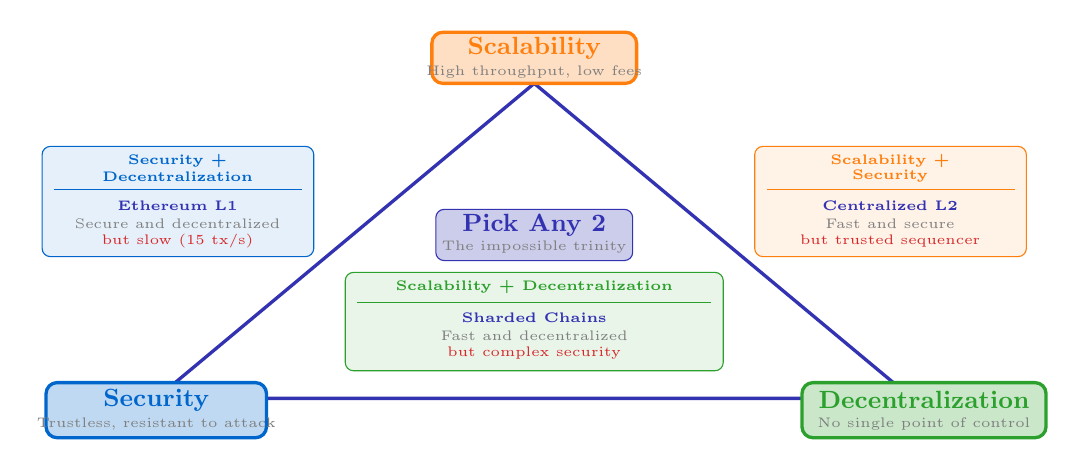
\begin{tikzpicture}
  % Main triangle
  \draw[very thick, mlpurple] (6.3,4.5) -- (1.5,0.5) -- (11.1,0.5) -- cycle;

  % Vertex labels
  % Top: Scalability
  \draw[fill=mlorange!25, draw=mlorange, very thick, rounded corners=4pt] (5.0,4.5) rectangle (7.6,5.15);
  \node[font=\small\bfseries, mlorange, align=center] at (6.3,4.95) {Scalability};
  \node[font=\tiny, mlgray, align=center] at (6.3,4.65) {High throughput, low fees};

  % Bottom-left: Security
  \draw[fill=mlblue!25, draw=mlblue, very thick, rounded corners=4pt] (0.1,0.0) rectangle (2.9,0.7);
  \node[font=\small\bfseries, mlblue, align=center] at (1.5,0.48) {Security};
  \node[font=\tiny, mlgray, align=center] at (1.5,0.18) {Trustless, resistant to attack};

  % Bottom-right: Decentralization
  \draw[fill=mlgreen!25, draw=mlgreen, very thick, rounded corners=4pt] (9.7,0.0) rectangle (12.8,0.7);
  \node[font=\small\bfseries, mlgreen, align=center] at (11.25,0.48) {Decentralization};
  \node[font=\tiny, mlgray, align=center] at (11.25,0.18) {No single point of control};

  % Center label
  \draw[fill=mllavender3, draw=mlpurple, rounded corners=3pt] (5.05,2.25) rectangle (7.55,2.9);
  \node[font=\small\bfseries, mlpurple, align=center] at (6.3,2.7) {Pick Any 2};
  \node[font=\tiny, mlgray, align=center] at (6.3,2.42) {The impossible trinity};

  % Side annotations
  % Left side: Security + Decentralization = Ethereum L1
  \draw[fill=mlblue!10, draw=mlblue, rounded corners=3pt] (0.05,2.3) rectangle (3.5,3.7);
  \node[font=\tiny\bfseries, mlblue, align=center] at (1.77,3.52) {Security +};
  \node[font=\tiny\bfseries, mlblue, align=center] at (1.77,3.32) {Decentralization};
  \draw[mlblue, thin] (0.2,3.15) -- (3.35,3.15);
  \node[font=\tiny\bfseries, mlpurple, align=center] at (1.77,2.95) {Ethereum L1};
  \node[font=\tiny, mlgray, align=center] at (1.77,2.72) {Secure and decentralized};
  \node[font=\tiny, mlred, align=center] at (1.77,2.5) {but slow (15 tx/s)};

  % Right side: Scalability + Security = Centralized L2
  \draw[fill=mlorange!10, draw=mlorange, rounded corners=3pt] (9.1,2.3) rectangle (12.55,3.7);
  \node[font=\tiny\bfseries, mlorange, align=center] at (10.82,3.52) {Scalability +};
  \node[font=\tiny\bfseries, mlorange, align=center] at (10.82,3.32) {Security};
  \draw[mlorange, thin] (9.25,3.15) -- (12.4,3.15);
  \node[font=\tiny\bfseries, mlpurple, align=center] at (10.82,2.95) {Centralized L2};
  \node[font=\tiny, mlgray, align=center] at (10.82,2.72) {Fast and secure};
  \node[font=\tiny, mlred, align=center] at (10.82,2.5) {but trusted sequencer};

  % Bottom: Scalability + Decentralization = Sharded Chains
  \draw[fill=mlgreen!10, draw=mlgreen, rounded corners=3pt] (3.9,0.85) rectangle (8.7,2.1);
  \node[font=\tiny\bfseries, mlgreen, align=center] at (6.3,1.92) {Scalability + Decentralization};
  \draw[mlgreen, thin] (4.05,1.72) -- (8.55,1.72);
  \node[font=\tiny\bfseries, mlpurple, align=center] at (6.3,1.52) {Sharded Chains};
  \node[font=\tiny, mlgray, align=center] at (6.3,1.3) {Fast and decentralized};
  \node[font=\tiny, mlred, align=center] at (6.3,1.08) {but complex security};
\end{tikzpicture}

\bottomnote{The blockchain trilemma: no system can simultaneously achieve scalability, security, and decentralization. Every blockchain design makes tradeoffs. L2 solutions help by inheriting L1 security.}
\end{frame}

% Frame 4: What is Layer 2?
\begin{frame}{What is Layer 2?}
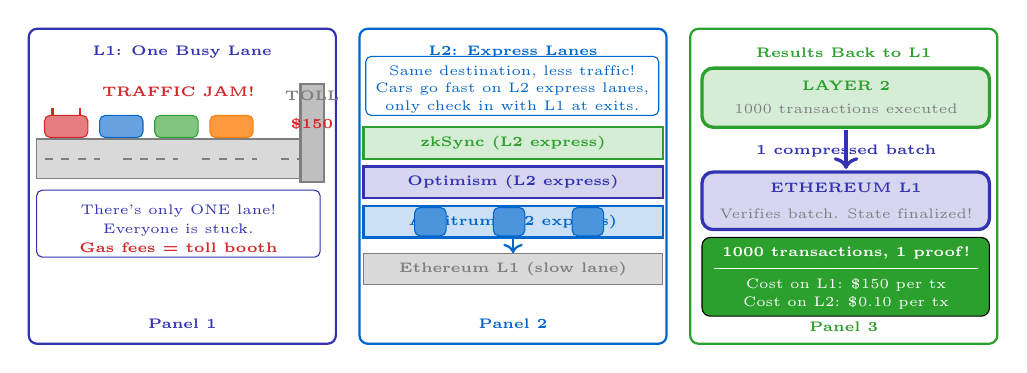
\begin{tikzpicture}
  % Panel borders
  \draw[thick, mlpurple, rounded corners=3pt] (0.1,0.2) rectangle (4.0,4.2);
  \draw[thick, mlblue,   rounded corners=3pt] (4.3,0.2) rectangle (8.2,4.2);
  \draw[thick, mlgreen,  rounded corners=3pt] (8.5,0.2) rectangle (12.4,4.2);

  % --- Panel 1: Busy highway (L1) ---
  \node[font=\tiny\bfseries, mlpurple] at (2.05,3.9) {L1: One Busy Lane};
  % Road
  \draw[fill=mlgray!30, draw=mlgray] (0.2,2.3) rectangle (3.8,2.8);
  % Dashed center line
  \draw[mlgray, dashed, thick] (0.3,2.55) -- (1.0,2.55);
  \draw[mlgray, dashed, thick] (1.3,2.55) -- (2.0,2.55);
  \draw[mlgray, dashed, thick] (2.3,2.55) -- (3.0,2.55);
  \draw[mlgray, dashed, thick] (3.3,2.55) -- (3.7,2.55);
  % Car 1
  \draw[fill=mlred!60, draw=mlred, rounded corners=2pt] (0.3,2.82) rectangle (0.85,3.1);
  \draw[mlred, thick] (0.4,3.1) -- (0.4,3.2);
  \draw[mlred, thick] (0.75,3.1) -- (0.75,3.2);
  % Car 2 (stopped)
  \draw[fill=mlblue!60, draw=mlblue, rounded corners=2pt] (1.0,2.82) rectangle (1.55,3.1);
  % Car 3
  \draw[fill=mlgreen!60, draw=mlgreen, rounded corners=2pt] (1.7,2.82) rectangle (2.25,3.1);
  % Car 4
  \draw[fill=mlorange!80, draw=mlorange, rounded corners=2pt] (2.4,2.82) rectangle (2.95,3.1);
  % Traffic jam label
  \node[font=\tiny\bfseries, mlred, align=center] at (2.0,3.4) {TRAFFIC JAM!};
  % Toll booth
  \draw[fill=mlgray!50, draw=mlgray, thick] (3.55,2.25) rectangle (3.85,3.5);
  \node[font=\tiny\bfseries, mlgray, align=center] at (3.7,3.35) {TOLL};
  \node[font=\tiny\bfseries, mlred, align=center] at (3.7,3.0) {\$150};
  % Speech bubble
  \draw[fill=white, draw=mlpurple, rounded corners=2pt] (0.2,1.3) rectangle (3.8,2.15);
  \node[font=\tiny, mlpurple, align=center] at (2.0,1.88) {There's only ONE lane!};
  \node[font=\tiny, mlpurple, align=center] at (2.0,1.65) {Everyone is stuck.};
  \node[font=\tiny\bfseries, mlred, align=center] at (2.0,1.42) {Gas fees = toll booth};
  \node[font=\tiny\bfseries, mlpurple] at (2.05,0.45) {Panel 1};

  % --- Panel 2: L2 express lanes ---
  \node[font=\tiny\bfseries, mlblue] at (6.25,3.9) {L2: Express Lanes};
  % L1 road (bottom)
  \draw[fill=mlgray!30, draw=mlgray] (4.35,0.95) rectangle (8.15,1.35);
  \node[font=\tiny\bfseries, mlgray, align=center] at (6.25,1.15) {Ethereum L1 (slow lane)};
  % L2 roads above (faster)
  \draw[fill=mlblue!20, draw=mlblue, thick] (4.35,1.55) rectangle (8.15,1.95);
  \node[font=\tiny\bfseries, mlblue, align=center] at (6.25,1.75) {Arbitrum (L2 express)};
  \draw[fill=mlpurple!20, draw=mlpurple, thick] (4.35,2.05) rectangle (8.15,2.45);
  \node[font=\tiny\bfseries, mlpurple, align=center] at (6.25,2.25) {Optimism (L2 express)};
  \draw[fill=mlgreen!20, draw=mlgreen, thick] (4.35,2.55) rectangle (8.15,2.95);
  \node[font=\tiny\bfseries, mlgreen, align=center] at (6.25,2.75) {zkSync (L2 express)};
  % Fast cars on L2
  \draw[fill=mlblue!70, draw=mlblue, rounded corners=2pt] (5.0,1.57) rectangle (5.4,1.93);
  \draw[fill=mlblue!70, draw=mlblue, rounded corners=2pt] (6.0,1.57) rectangle (6.4,1.93);
  \draw[fill=mlblue!70, draw=mlblue, rounded corners=2pt] (7.0,1.57) rectangle (7.4,1.93);
  % Exit ramps to L1
  \draw[->, thick, mlblue] (6.25,1.55) -- (6.25,1.35);
  % Speech bubble
  \draw[fill=white, draw=mlblue, rounded corners=2pt] (4.38,3.1) rectangle (8.1,3.85);
  \node[font=\tiny, mlblue, align=center] at (6.24,3.65) {Same destination, less traffic!};
  \node[font=\tiny, mlblue, align=center] at (6.24,3.43) {Cars go fast on L2 express lanes,};
  \node[font=\tiny, mlblue, align=center] at (6.24,3.21) {only check in with L1 at exits.};
  \node[font=\tiny\bfseries, mlblue] at (6.25,0.45) {Panel 2};

  % --- Panel 3: Summary posted to L1 ---
  \node[font=\tiny\bfseries, mlgreen] at (10.45,3.9) {Results Back to L1};
  % L2 box
  \draw[fill=mlgreen!20, draw=mlgreen, very thick, rounded corners=4pt] (8.65,2.95) rectangle (12.3,3.7);
  \node[font=\tiny\bfseries, mlgreen, align=center] at (10.48,3.48) {LAYER 2};
  \node[font=\tiny, mlgray, align=center] at (10.48,3.18) {1000 transactions executed};
  % Arrow down
  \draw[->, very thick, mlpurple] (10.48,2.92) -- (10.48,2.42);
  \node[font=\tiny\bfseries, mlpurple, align=center] at (10.48,2.65) {1 compressed batch};
  % L1 box
  \draw[fill=mlpurple!20, draw=mlpurple, very thick, rounded corners=4pt] (8.65,1.65) rectangle (12.3,2.38);
  \node[font=\tiny\bfseries, mlpurple, align=center] at (10.48,2.18) {ETHEREUM L1};
  \node[font=\tiny, mlgray, align=center] at (10.48,1.85) {Verifies batch. State finalized!};
  % Result box
  \draw[fill=mlgreen, rounded corners=3pt] (8.65,0.55) rectangle (12.3,1.55);
  \node[font=\tiny\bfseries, white, align=center] at (10.48,1.35) {1000 transactions, 1 proof!};
  \draw[white, thin] (8.8,1.15) -- (12.15,1.15);
  \node[font=\tiny, white, align=center] at (10.48,0.95) {Cost on L1: \$150 per tx};
  \node[font=\tiny, white, align=center] at (10.48,0.72) {Cost on L2: \$0.10 per tx};
  \node[font=\tiny\bfseries, mlgreen] at (10.45,0.42) {Panel 3};
\end{tikzpicture}

\bottomnote{Layer 2 is a secondary protocol built on top of L1. It executes transactions off-chain at high speed and low cost, then posts compressed results back to L1 for security and finality.}
\end{frame}

% Frame 5: Types of Layer 2 Solutions
\begin{frame}{Types of Layer 2 Solutions}
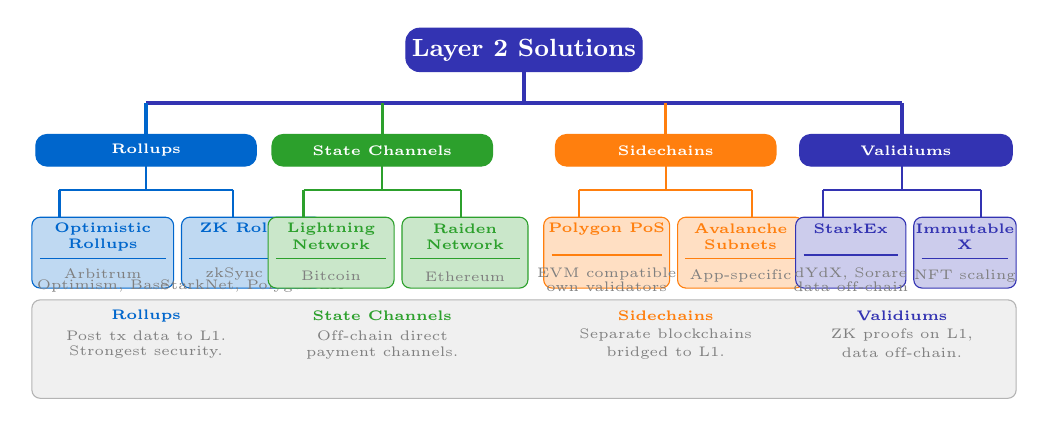
\begin{tikzpicture}
  % Root node
  \draw[fill=mlpurple, draw=mlpurple, rounded corners=5pt] (4.8,4.45) rectangle (7.8,5.0);
  \node[font=\small\bfseries, white, align=center] at (6.3,4.72) {Layer 2 Solutions};

  % Root stem down
  \draw[very thick, mlpurple] (6.3,4.45) -- (6.3,4.05);
  % Horizontal bar
  \draw[very thick, mlpurple] (1.5,4.05) -- (11.1,4.05);

  % Branch 1 (left): Rollups (mlblue)
  \draw[very thick, mlblue] (1.5,4.05) -- (1.5,3.65);
  \draw[fill=mlblue, draw=mlblue, rounded corners=4pt] (0.1,3.25) rectangle (2.9,3.65);
  \node[font=\tiny\bfseries, white, align=center] at (1.5,3.45) {Rollups};

  % Rollup sub-branches
  \draw[thick, mlblue] (1.5,3.25) -- (1.5,2.95);
  \draw[thick, mlblue] (0.4,2.95) -- (2.6,2.95);
  \draw[thick, mlblue] (0.4,2.95) -- (0.4,2.6);
  \draw[thick, mlblue] (2.6,2.95) -- (2.6,2.6);
  \draw[fill=mlblue!25, draw=mlblue, rounded corners=3pt] (0.05,1.7) rectangle (1.85,2.6);
  \node[font=\tiny\bfseries, mlblue, align=center] at (0.95,2.45) {Optimistic};
  \node[font=\tiny\bfseries, mlblue, align=center] at (0.95,2.25) {Rollups};
  \draw[mlblue, thin] (0.15,2.08) -- (1.75,2.08);
  \node[font=\tiny, mlgray, align=center] at (0.95,1.88) {Arbitrum};
  \node[font=\tiny, mlgray, align=center] at (0.95,1.72) {Optimism, Base};
  \draw[fill=mlblue!25, draw=mlblue, rounded corners=3pt] (1.95,1.7) rectangle (3.75,2.6);
  \node[font=\tiny\bfseries, mlblue, align=center] at (2.85,2.45) {ZK Rollups};
  \draw[mlblue, thin] (2.05,2.08) -- (3.65,2.08);
  \node[font=\tiny, mlgray, align=center] at (2.85,1.88) {zkSync Era};
  \node[font=\tiny, mlgray, align=center] at (2.85,1.72) {StarkNet, Polygon ZK};

  % Branch 2: State Channels (mlgreen)
  \draw[very thick, mlgreen] (4.5,4.05) -- (4.5,3.65);
  \draw[fill=mlgreen, draw=mlgreen, rounded corners=4pt] (3.1,3.25) rectangle (5.9,3.65);
  \node[font=\tiny\bfseries, white, align=center] at (4.5,3.45) {State Channels};

  % State channel sub-branches
  \draw[thick, mlgreen] (4.5,3.25) -- (4.5,2.95);
  \draw[thick, mlgreen] (3.5,2.95) -- (5.5,2.95);
  \draw[thick, mlgreen] (3.5,2.95) -- (3.5,2.6);
  \draw[thick, mlgreen] (5.5,2.95) -- (5.5,2.6);
  \draw[fill=mlgreen!25, draw=mlgreen, rounded corners=3pt] (3.05,1.7) rectangle (4.65,2.6);
  \node[font=\tiny\bfseries, mlgreen, align=center] at (3.85,2.45) {Lightning};
  \node[font=\tiny\bfseries, mlgreen, align=center] at (3.85,2.25) {Network};
  \draw[mlgreen, thin] (3.15,2.08) -- (4.55,2.08);
  \node[font=\tiny, mlgray, align=center] at (3.85,1.85) {Bitcoin};
  \draw[fill=mlgreen!25, draw=mlgreen, rounded corners=3pt] (4.75,1.7) rectangle (6.35,2.6);
  \node[font=\tiny\bfseries, mlgreen, align=center] at (5.55,2.45) {Raiden};
  \node[font=\tiny\bfseries, mlgreen, align=center] at (5.55,2.25) {Network};
  \draw[mlgreen, thin] (4.85,2.08) -- (6.25,2.08);
  \node[font=\tiny, mlgray, align=center] at (5.55,1.85) {Ethereum};

  % Branch 3: Sidechains (mlorange)
  \draw[very thick, mlorange] (8.1,4.05) -- (8.1,3.65);
  \draw[fill=mlorange, draw=mlorange, rounded corners=4pt] (6.7,3.25) rectangle (9.5,3.65);
  \node[font=\tiny\bfseries, white, align=center] at (8.1,3.45) {Sidechains};

  % Sidechain sub-branches
  \draw[thick, mlorange] (8.1,3.25) -- (8.1,2.95);
  \draw[thick, mlorange] (7.0,2.95) -- (9.2,2.95);
  \draw[thick, mlorange] (7.0,2.95) -- (7.0,2.6);
  \draw[thick, mlorange] (9.2,2.95) -- (9.2,2.6);
  \draw[fill=mlorange!25, draw=mlorange, rounded corners=3pt] (6.55,1.7) rectangle (8.15,2.6);
  \node[font=\tiny\bfseries, mlorange, align=center] at (7.35,2.45) {Polygon PoS};
  \draw[mlorange, thin] (6.65,2.12) -- (8.05,2.12);
  \node[font=\tiny, mlgray, align=center] at (7.35,1.88) {EVM compatible};
  \node[font=\tiny, mlgray, align=center] at (7.35,1.72) {own validators};
  \draw[fill=mlorange!25, draw=mlorange, rounded corners=3pt] (8.25,1.7) rectangle (9.85,2.6);
  \node[font=\tiny\bfseries, mlorange, align=center] at (9.05,2.45) {Avalanche};
  \node[font=\tiny\bfseries, mlorange, align=center] at (9.05,2.25) {Subnets};
  \draw[mlorange, thin] (8.35,2.08) -- (9.75,2.08);
  \node[font=\tiny, mlgray, align=center] at (9.05,1.85) {App-specific};

  % Branch 4: Validiums (mlpurple)
  \draw[very thick, mlpurple] (11.1,4.05) -- (11.1,3.65);
  \draw[fill=mlpurple, draw=mlpurple, rounded corners=4pt] (9.8,3.25) rectangle (12.5,3.65);
  \node[font=\tiny\bfseries, white, align=center] at (11.15,3.45) {Validiums};

  % Validium sub-branches
  \draw[thick, mlpurple] (11.1,3.25) -- (11.1,2.95);
  \draw[thick, mlpurple] (10.1,2.95) -- (12.1,2.95);
  \draw[thick, mlpurple] (10.1,2.95) -- (10.1,2.6);
  \draw[thick, mlpurple] (12.1,2.95) -- (12.1,2.6);
  \draw[fill=mlpurple!25, draw=mlpurple, rounded corners=3pt] (9.75,1.7) rectangle (11.15,2.6);
  \node[font=\tiny\bfseries, mlpurple, align=center] at (10.45,2.45) {StarkEx};
  \draw[mlpurple, thin] (9.85,2.12) -- (11.05,2.12);
  \node[font=\tiny, mlgray, align=center] at (10.45,1.88) {dYdX, Sorare};
  \node[font=\tiny, mlgray, align=center] at (10.45,1.72) {data off-chain};
  \draw[fill=mlpurple!25, draw=mlpurple, rounded corners=3pt] (11.25,1.7) rectangle (12.55,2.6);
  \node[font=\tiny\bfseries, mlpurple, align=center] at (11.9,2.45) {Immutable};
  \node[font=\tiny\bfseries, mlpurple, align=center] at (11.9,2.25) {X};
  \draw[mlpurple, thin] (11.35,2.08) -- (12.45,2.08);
  \node[font=\tiny, mlgray, align=center] at (11.9,1.85) {NFT scaling};

  % Description boxes at bottom
  \draw[fill=lightgray, draw=midgray, rounded corners=3pt] (0.05,0.3) rectangle (12.55,1.55);
  \node[font=\tiny\bfseries, mlblue, align=center] at (1.5,1.35) {Rollups};
  \node[font=\tiny, mlgray, align=center] at (1.5,1.1) {Post tx data to L1.};
  \node[font=\tiny, mlgray, align=center] at (1.5,0.88) {Strongest security.};
  \node[font=\tiny\bfseries, mlgreen, align=center] at (4.5,1.35) {State Channels};
  \node[font=\tiny, mlgray, align=center] at (4.5,1.1) {Off-chain direct};
  \node[font=\tiny, mlgray, align=center] at (4.5,0.88) {payment channels.};
  \node[font=\tiny\bfseries, mlorange, align=center] at (8.1,1.35) {Sidechains};
  \node[font=\tiny, mlgray, align=center] at (8.1,1.1) {Separate blockchains};
  \node[font=\tiny, mlgray, align=center] at (8.1,0.88) {bridged to L1.};
  \node[font=\tiny\bfseries, mlpurple, align=center] at (11.1,1.35) {Validiums};
  \node[font=\tiny, mlgray, align=center] at (11.1,1.1) {ZK proofs on L1,};
  \node[font=\tiny, mlgray, align=center] at (11.1,0.88) {data off-chain.};
\end{tikzpicture}

\bottomnote{Four main L2 categories: Rollups (strongest security, data on L1), State Channels (peer-to-peer, for repeated interactions), Sidechains (own consensus, bridged to L1), Validiums (ZK proofs on L1, data off-chain).}
\end{frame}

% Frame 6: Optimistic vs ZK Rollups
\begin{frame}{Optimistic vs.\ ZK Rollups}
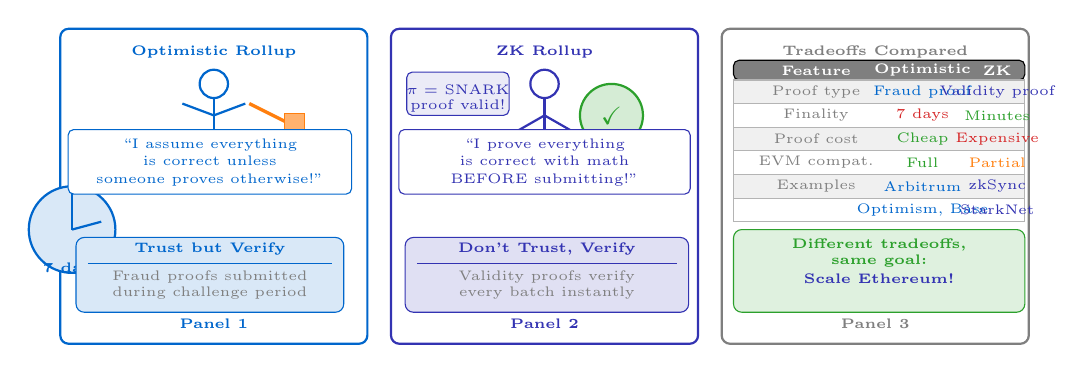
\begin{tikzpicture}
  % Panel borders
  \draw[thick, mlblue,   rounded corners=3pt] (0.1,0.2) rectangle (4.0,4.2);
  \draw[thick, mlpurple, rounded corners=3pt] (4.3,0.2) rectangle (8.2,4.2);
  \draw[thick, mlgray,   rounded corners=3pt] (8.5,0.2) rectangle (12.4,4.2);

  % --- Panel 1: Optimistic Rollup ---
  \node[font=\tiny\bfseries, mlblue] at (2.05,3.9) {Optimistic Rollup};
  % Judge stick figure (relaxed)
  \draw[mlblue,thick] (2.05,3.5) circle (0.18);
  \draw[mlblue,thick] (2.05,3.32) -- (2.05,2.88);
  \draw[mlblue,thick] (2.05,3.1) -- (1.65,3.25);
  \draw[mlblue,thick] (2.05,3.1) -- (2.45,3.25);
  \draw[mlblue,thick] (2.05,2.88) -- (1.82,2.60);
  \draw[mlblue,thick] (2.05,2.88) -- (2.28,2.60);
  \node[font=\tiny, mlblue] at (2.05,2.45) {Judge};
  % Gavel
  \draw[mlorange, very thick] (2.5,3.25) -- (3.0,3.0);
  \draw[fill=mlorange!60, draw=mlorange] (2.95,3.12) rectangle (3.2,2.88);
  % 7-day clock
  \draw[fill=mlblue!15, draw=mlblue, thick] (0.25,1.65) circle (0.55);
  \draw[mlblue, thick] (0.25,1.65) -- (0.25,2.12);
  \draw[mlblue, thick] (0.25,1.65) -- (0.62,1.75);
  \node[font=\tiny\bfseries, mlblue, align=center] at (0.25,1.15) {7 days};
  % Speech bubble
  \draw[fill=white, draw=mlblue, rounded corners=2pt] (0.2,2.1) rectangle (3.8,2.92);
  \node[font=\tiny, mlblue, align=center] at (2.0,2.72) {``I assume everything};
  \node[font=\tiny, mlblue, align=center] at (2.0,2.52) {is correct unless};
  \node[font=\tiny, mlblue, align=center] at (2.0,2.28) {someone proves otherwise!''};
  % Labels
  \draw[fill=mlblue!15, draw=mlblue, rounded corners=3pt] (0.3,0.6) rectangle (3.7,1.55);
  \node[font=\tiny\bfseries, mlblue, align=center] at (2.0,1.4) {Trust but Verify};
  \draw[mlblue, thin] (0.45,1.22) -- (3.55,1.22);
  \node[font=\tiny, mlgray, align=center] at (2.0,1.05) {Fraud proofs submitted};
  \node[font=\tiny, mlgray, align=center] at (2.0,0.85) {during challenge period};
  \node[font=\tiny\bfseries, mlblue] at (2.05,0.45) {Panel 1};

  % --- Panel 2: ZK Rollup ---
  \node[font=\tiny\bfseries, mlpurple] at (6.25,3.9) {ZK Rollup};
  % Scientist stick figure
  \draw[mlpurple,thick] (6.25,3.5) circle (0.18);
  \draw[mlpurple,thick] (6.25,3.32) -- (6.25,2.88);
  \draw[mlpurple,thick] (6.25,3.1) -- (5.9,2.9);
  \draw[mlpurple,thick] (6.25,3.1) -- (6.6,2.9);
  \draw[mlpurple,thick] (6.25,2.88) -- (6.02,2.60);
  \draw[mlpurple,thick] (6.25,2.88) -- (6.48,2.60);
  \node[font=\tiny, mlpurple] at (6.25,2.45) {Prover};
  % Math equation
  \draw[fill=mlpurple!10, draw=mlpurple, rounded corners=2pt] (4.5,3.1) rectangle (5.8,3.65);
  \node[font=\tiny, mlpurple, align=center] at (5.15,3.42) {$\pi = $ SNARK};
  \node[font=\tiny, mlpurple, align=center] at (5.15,3.22) {proof valid!};
  % Instant checkmark
  \draw[fill=mlgreen!20, draw=mlgreen, thick] (7.1,3.1) circle (0.4);
  \node[font=\small\bfseries, mlgreen] at (7.1,3.1) {\checkmark};
  \node[font=\tiny\bfseries, mlgreen, align=center] at (7.1,2.6) {Instant!};
  % Speech bubble
  \draw[fill=white, draw=mlpurple, rounded corners=2pt] (4.4,2.1) rectangle (8.1,2.92);
  \node[font=\tiny, mlpurple, align=center] at (6.25,2.72) {``I prove everything};
  \node[font=\tiny, mlpurple, align=center] at (6.25,2.52) {is correct with math};
  \node[font=\tiny, mlpurple, align=center] at (6.25,2.28) {BEFORE submitting!''};
  % Labels
  \draw[fill=mlpurple!15, draw=mlpurple, rounded corners=3pt] (4.48,0.6) rectangle (8.08,1.55);
  \node[font=\tiny\bfseries, mlpurple, align=center] at (6.28,1.4) {Don't Trust, Verify};
  \draw[mlpurple, thin] (4.63,1.22) -- (7.93,1.22);
  \node[font=\tiny, mlgray, align=center] at (6.28,1.05) {Validity proofs verify};
  \node[font=\tiny, mlgray, align=center] at (6.28,0.85) {every batch instantly};
  \node[font=\tiny\bfseries, mlpurple] at (6.25,0.45) {Panel 2};

  % --- Panel 3: Comparison ---
  \node[font=\tiny\bfseries, mlgray] at (10.45,3.9) {Tradeoffs Compared};
  % Table header
  \draw[fill=mlgray, rounded corners=2pt] (8.65,3.55) rectangle (12.35,3.8);
  \node[font=\tiny\bfseries, white, align=center] at (9.7,3.67) {Feature};
  \node[font=\tiny\bfseries, white, align=center] at (11.05,3.67) {Optimistic};
  \node[font=\tiny\bfseries, white, align=center] at (12.0,3.67) {ZK};
  % Row 1
  \draw[fill=lightgray, draw=midgray] (8.65,3.25) rectangle (12.35,3.55);
  \node[font=\tiny, mlgray, align=center] at (9.7,3.4) {Proof type};
  \node[font=\tiny, mlblue, align=center] at (11.05,3.4) {Fraud proof};
  \node[font=\tiny, mlpurple, align=center] at (12.0,3.4) {Validity proof};
  % Row 2
  \draw[fill=white, draw=midgray] (8.65,2.95) rectangle (12.35,3.25);
  \node[font=\tiny, mlgray, align=center] at (9.7,3.1) {Finality};
  \node[font=\tiny, mlred, align=center] at (11.05,3.1) {7 days};
  \node[font=\tiny, mlgreen, align=center] at (12.0,3.1) {Minutes};
  % Row 3
  \draw[fill=lightgray, draw=midgray] (8.65,2.65) rectangle (12.35,2.95);
  \node[font=\tiny, mlgray, align=center] at (9.7,2.8) {Proof cost};
  \node[font=\tiny, mlgreen, align=center] at (11.05,2.8) {Cheap};
  \node[font=\tiny, mlred, align=center] at (12.0,2.8) {Expensive};
  % Row 4
  \draw[fill=white, draw=midgray] (8.65,2.35) rectangle (12.35,2.65);
  \node[font=\tiny, mlgray, align=center] at (9.7,2.5) {EVM compat.};
  \node[font=\tiny, mlgreen, align=center] at (11.05,2.5) {Full};
  \node[font=\tiny, mlorange, align=center] at (12.0,2.5) {Partial};
  % Row 5
  \draw[fill=lightgray, draw=midgray] (8.65,2.05) rectangle (12.35,2.35);
  \node[font=\tiny, mlgray, align=center] at (9.7,2.2) {Examples};
  \node[font=\tiny, mlblue, align=center] at (11.05,2.2) {Arbitrum};
  \node[font=\tiny, mlpurple, align=center] at (12.0,2.2) {zkSync};
  % Row 6
  \draw[fill=white, draw=midgray] (8.65,1.75) rectangle (12.35,2.05);
  \node[font=\tiny, mlgray, align=center] at (9.7,1.9) {};
  \node[font=\tiny, mlblue, align=center] at (11.05,1.9) {Optimism, Base};
  \node[font=\tiny, mlpurple, align=center] at (12.0,1.9) {StarkNet};
  % Bottom note box
  \draw[fill=mlgreen!15, draw=mlgreen, rounded corners=3pt] (8.65,0.6) rectangle (12.35,1.65);
  \node[font=\tiny\bfseries, mlgreen, align=center] at (10.5,1.45) {Different tradeoffs,};
  \node[font=\tiny\bfseries, mlgreen, align=center] at (10.5,1.25) {same goal:};
  \node[font=\tiny\bfseries, mlpurple, align=center] at (10.5,1.02) {Scale Ethereum!};
  \node[font=\tiny\bfseries, mlgray] at (10.45,0.45) {Panel 3};
\end{tikzpicture}

\bottomnote{Optimistic rollups assume validity and use fraud proofs (7-day withdrawal delay). ZK rollups prove validity cryptographically with SNARKs/STARKs (instant finality, higher proving cost).}
\end{frame}

% Frame 7: How Rollups Work
\begin{frame}{How Rollups Work: Step by Step}
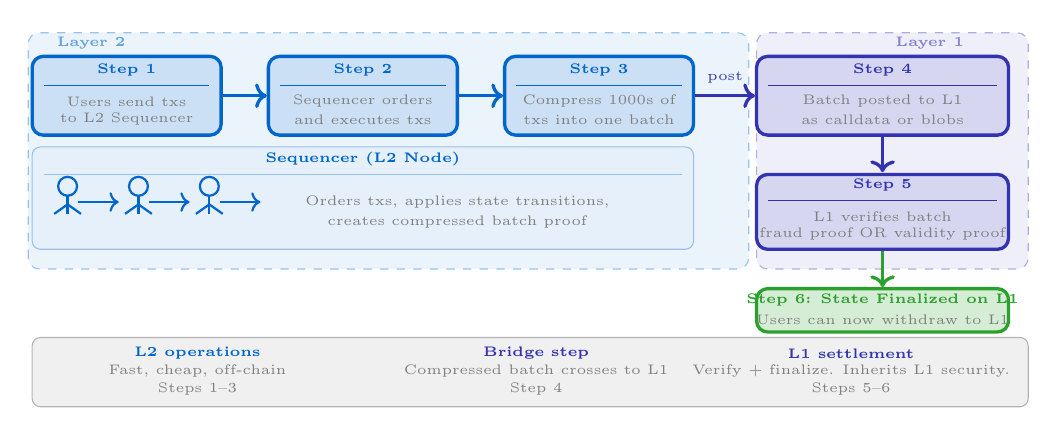
\begin{tikzpicture}
  % Background: L2 zone vs L1 zone
  \draw[fill=mlblue!8, draw=mlblue!40, rounded corners=4pt, dashed] (0.05,1.85) rectangle (9.2,4.85);
  \node[font=\tiny\bfseries, mlblue!60, align=center] at (0.85,4.72) {Layer 2};

  \draw[fill=mlpurple!8, draw=mlpurple!40, rounded corners=4pt, dashed] (9.3,1.85) rectangle (12.75,4.85);
  \node[font=\tiny\bfseries, mlpurple!60, align=center] at (11.5,4.72) {Layer 1};

  % Step 1: Users send transactions
  \draw[fill=mlblue!20, draw=mlblue, very thick, rounded corners=4pt] (0.1,3.55) rectangle (2.5,4.55);
  \node[font=\tiny\bfseries, mlblue, align=center] at (1.3,4.38) {Step 1};
  \draw[mlblue, thin] (0.25,4.18) -- (2.35,4.18);
  \node[font=\tiny, mlgray, align=center] at (1.3,3.98) {Users send txs};
  \node[font=\tiny, mlgray, align=center] at (1.3,3.75) {to L2 Sequencer};

  % Arrow 1 -> 2
  \draw[->, very thick, mlblue] (2.52,4.05) -- (3.08,4.05);

  % Step 2: Sequencer orders and executes
  \draw[fill=mlblue!20, draw=mlblue, very thick, rounded corners=4pt] (3.1,3.55) rectangle (5.5,4.55);
  \node[font=\tiny\bfseries, mlblue, align=center] at (4.3,4.38) {Step 2};
  \draw[mlblue, thin] (3.25,4.18) -- (5.35,4.18);
  \node[font=\tiny, mlgray, align=center] at (4.3,3.98) {Sequencer orders};
  \node[font=\tiny, mlgray, align=center] at (4.3,3.75) {and executes txs};

  % Arrow 2 -> 3
  \draw[->, very thick, mlblue] (5.52,4.05) -- (6.08,4.05);

  % Step 3: Batch txs
  \draw[fill=mlblue!20, draw=mlblue, very thick, rounded corners=4pt] (6.1,3.55) rectangle (8.5,4.55);
  \node[font=\tiny\bfseries, mlblue, align=center] at (7.3,4.38) {Step 3};
  \draw[mlblue, thin] (6.25,4.18) -- (8.35,4.18);
  \node[font=\tiny, mlgray, align=center] at (7.3,3.98) {Compress 1000s of};
  \node[font=\tiny, mlgray, align=center] at (7.3,3.75) {txs into one batch};

  % Arrow 3 -> 4 (crosses L1/L2 boundary)
  \draw[->, very thick, mlpurple] (8.52,4.05) -- (9.28,4.05);
  \node[font=\tiny, mlpurple, align=center] at (8.9,4.28) {post};

  % Step 4: Post to L1
  \draw[fill=mlpurple!20, draw=mlpurple, very thick, rounded corners=4pt] (9.3,3.55) rectangle (12.5,4.55);
  \node[font=\tiny\bfseries, mlpurple, align=center] at (10.9,4.38) {Step 4};
  \draw[mlpurple, thin] (9.45,4.18) -- (12.35,4.18);
  \node[font=\tiny, mlgray, align=center] at (10.9,3.98) {Batch posted to L1};
  \node[font=\tiny, mlgray, align=center] at (10.9,3.75) {as calldata or blobs};

  % Arrow Step 4 -> Step 5 (downward in L1 zone)
  \draw[->, very thick, mlpurple] (10.9,3.53) -- (10.9,3.08);

  % Step 5: L1 verifies
  \draw[fill=mlpurple!20, draw=mlpurple, very thick, rounded corners=4pt] (9.3,2.1) rectangle (12.5,3.05);
  \node[font=\tiny\bfseries, mlpurple, align=center] at (10.9,2.92) {Step 5};
  \draw[mlpurple, thin] (9.45,2.72) -- (12.35,2.72);
  \node[font=\tiny, mlgray, align=center] at (10.9,2.52) {L1 verifies batch};
  \node[font=\tiny, mlgray, align=center] at (10.9,2.3) {fraud proof OR validity proof};

  % Arrow Step 5 -> Step 6 (back in L1 zone going down)
  \draw[->, very thick, mlgreen] (10.9,2.08) -- (10.9,1.62);

  % Step 6: State finalized
  \draw[fill=mlgreen!20, draw=mlgreen, very thick, rounded corners=4pt] (9.3,1.05) rectangle (12.5,1.6);
  \node[font=\tiny\bfseries, mlgreen, align=center] at (10.9,1.45) {Step 6: State Finalized on L1};
  \node[font=\tiny, mlgray, align=center] at (10.9,1.2) {Users can now withdraw to L1};

  % User flow (bottom of L2 area, showing user side)
  \draw[fill=mlblue!10, draw=mlblue!40, rounded corners=3pt] (0.1,2.1) rectangle (8.5,3.4);
  \node[font=\tiny\bfseries, mlblue, align=center] at (4.3,3.25) {Sequencer (L2 Node)};
  \draw[mlblue!40, thin] (0.25,3.05) -- (8.35,3.05);
  % User icons with arrows
  \draw[mlblue,thick] (0.55,2.9) circle (0.12);
  \draw[mlblue,thick] (0.55,2.78) -- (0.55,2.55);
  \draw[mlblue,thick] (0.55,2.67) -- (0.38,2.55);
  \draw[mlblue,thick] (0.55,2.67) -- (0.72,2.55);
  \draw[->, thick, mlblue] (0.68,2.7) -- (1.2,2.7);

  \draw[mlblue,thick] (1.45,2.9) circle (0.12);
  \draw[mlblue,thick] (1.45,2.78) -- (1.45,2.55);
  \draw[mlblue,thick] (1.45,2.67) -- (1.28,2.55);
  \draw[mlblue,thick] (1.45,2.67) -- (1.62,2.55);
  \draw[->, thick, mlblue] (1.58,2.7) -- (2.1,2.7);

  \draw[mlblue,thick] (2.35,2.9) circle (0.12);
  \draw[mlblue,thick] (2.35,2.78) -- (2.35,2.55);
  \draw[mlblue,thick] (2.35,2.67) -- (2.18,2.55);
  \draw[mlblue,thick] (2.35,2.67) -- (2.52,2.55);
  \draw[->, thick, mlblue] (2.48,2.7) -- (3.0,2.7);

  \node[font=\tiny, mlgray, align=center] at (5.5,2.7) {Orders txs, applies state transitions,};
  \node[font=\tiny, mlgray, align=center] at (5.5,2.45) {creates compressed batch proof};

  % Legend box
  \draw[fill=lightgray, draw=midgray, rounded corners=3pt] (0.1,0.1) rectangle (12.75,0.98);
  \node[font=\tiny\bfseries, mlblue, align=center] at (2.2,0.78) {L2 operations};
  \node[font=\tiny, mlgray, align=center] at (2.2,0.55) {Fast, cheap, off-chain};
  \node[font=\tiny, mlgray, align=center] at (2.2,0.32) {Steps 1--3};
  \node[font=\tiny\bfseries, mlpurple, align=center] at (6.5,0.78) {Bridge step};
  \node[font=\tiny, mlgray, align=center] at (6.5,0.55) {Compressed batch crosses to L1};
  \node[font=\tiny, mlgray, align=center] at (6.5,0.32) {Step 4};
  \node[font=\tiny\bfseries, mlpurple, align=center] at (10.5,0.78) {L1 settlement};
  \node[font=\tiny, mlgray, align=center] at (10.5,0.55) {Verify + finalize. Inherits L1 security.};
  \node[font=\tiny, mlgray, align=center] at (10.5,0.32) {Steps 5--6};
\end{tikzpicture}

\bottomnote{Rollup flow: users submit txs to L2 sequencer (fast, cheap) $\to$ sequencer batches and compresses $\to$ batch posted to L1 $\to$ L1 verifies via fraud proof (Optimistic) or validity proof (ZK) $\to$ state finalized.}
\end{frame}

% Frame 8: Bridge Security Risks
\begin{frame}{Bridge Security Risks}
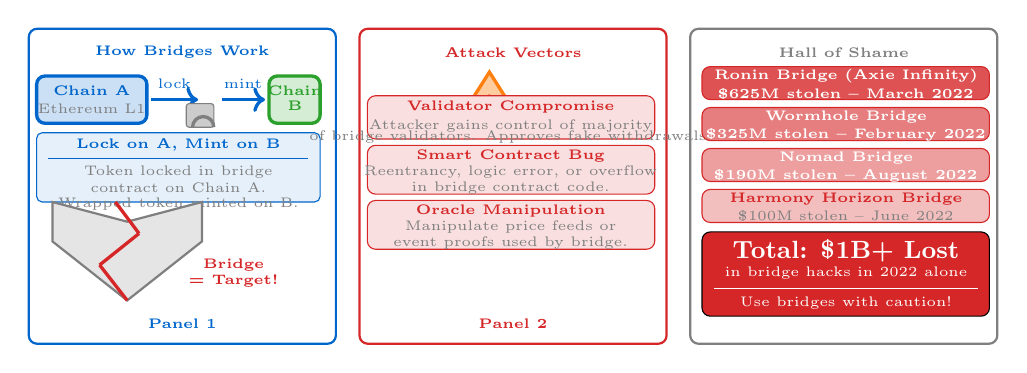
\begin{tikzpicture}
  % Panel borders
  \draw[thick, mlblue,   rounded corners=3pt] (0.1,0.2) rectangle (4.0,4.2);
  \draw[thick, mlred,    rounded corners=3pt] (4.3,0.2) rectangle (8.2,4.2);
  \draw[thick, mlgray,   rounded corners=3pt] (8.5,0.2) rectangle (12.4,4.2);

  % --- Panel 1: Bridge concept ---
  \node[font=\tiny\bfseries, mlblue] at (2.05,3.9) {How Bridges Work};
  % Chain A box
  \draw[fill=mlblue!20, draw=mlblue, very thick, rounded corners=3pt] (0.2,3.0) rectangle (1.6,3.6);
  \node[font=\tiny\bfseries, mlblue, align=center] at (0.9,3.42) {Chain A};
  \node[font=\tiny, mlgray, align=center] at (0.9,3.18) {Ethereum L1};
  % Lock arrow
  \draw[->, very thick, mlblue] (1.65,3.3) -- (2.25,3.3);
  \node[font=\tiny, mlblue, align=center] at (1.95,3.5) {lock};
  % Lock icon
  \draw[fill=mlgray!40, draw=mlgray, rounded corners=1pt] (2.1,2.95) rectangle (2.45,3.25);
  \draw[mlgray, very thick] (2.18,2.95) arc(180:0:0.135);
  % Bridge arrow
  \draw[->, very thick, mlblue] (2.55,3.3) -- (3.1,3.3);
  \node[font=\tiny, mlblue, align=center] at (2.82,3.5) {mint};
  % Chain B box
  \draw[fill=mlgreen!20, draw=mlgreen, very thick, rounded corners=3pt] (3.15,3.0) rectangle (3.8,3.6);
  \node[font=\tiny\bfseries, mlgreen, align=center] at (3.48,3.42) {Chain};
  \node[font=\tiny\bfseries, mlgreen, align=center] at (3.48,3.22) {B};
  % Explanation
  \draw[fill=mlblue!10, draw=mlblue, rounded corners=2pt] (0.2,2.0) rectangle (3.8,2.88);
  \node[font=\tiny\bfseries, mlblue, align=center] at (2.0,2.72) {Lock on A, Mint on B};
  \draw[mlblue, thin] (0.35,2.55) -- (3.65,2.55);
  \node[font=\tiny, mlgray, align=center] at (2.0,2.38) {Token locked in bridge};
  \node[font=\tiny, mlgray, align=center] at (2.0,2.18) {contract on Chain A.};
  \node[font=\tiny, mlgray, align=center] at (2.0,1.98) {Wrapped token minted on B.};
  % Cracked shield
  \draw[fill=mlgray!20, draw=mlgray, thick] (1.35,0.75) -- (0.4,1.5) -- (0.4,2.0) -- (1.35,1.75) -- (2.3,2.0) -- (2.3,1.5) -- cycle;
  \draw[mlred, very thick] (1.35,0.75) -- (1.0,1.2);
  \draw[mlred, very thick] (1.0,1.2) -- (1.5,1.6);
  \draw[mlred, very thick] (1.5,1.6) -- (1.2,2.0);
  \node[font=\tiny\bfseries, mlred, align=center] at (2.7,1.2) {Bridge};
  \node[font=\tiny\bfseries, mlred, align=center] at (2.7,1.0) {= Target!};
  \node[font=\tiny\bfseries, mlblue] at (2.05,0.45) {Panel 1};

  % --- Panel 2: Attack scenarios ---
  \node[font=\tiny\bfseries, mlred] at (6.25,3.9) {Attack Vectors};
  % Warning triangle
  \draw[fill=mlorange!40, draw=mlorange, very thick] (5.95,3.65) -- (5.6,3.1) -- (6.3,3.1) -- cycle;
  \node[font=\small\bfseries, mlred] at (5.95,3.25) {!};

  % Attack 1: Validator compromise
  \draw[fill=mlred!15, draw=mlred, rounded corners=3pt] (4.4,2.8) rectangle (8.05,3.35);
  \node[font=\tiny\bfseries, mlred, align=center] at (6.22,3.2) {Validator Compromise};
  \node[font=\tiny, mlgray, align=center] at (6.22,2.96) {Attacker gains control of majority};
  \node[font=\tiny, mlgray, align=center] at (6.22,2.82) {of bridge validators. Approves fake withdrawals.};

  % Attack 2: Smart contract bug
  \draw[fill=mlred!15, draw=mlred, rounded corners=3pt] (4.4,2.1) rectangle (8.05,2.72);
  \node[font=\tiny\bfseries, mlred, align=center] at (6.22,2.58) {Smart Contract Bug};
  \node[font=\tiny, mlgray, align=center] at (6.22,2.38) {Reentrancy, logic error, or overflow};
  \node[font=\tiny, mlgray, align=center] at (6.22,2.18) {in bridge contract code.};

  % Attack 3: Oracle manipulation
  \draw[fill=mlred!15, draw=mlred, rounded corners=3pt] (4.4,1.4) rectangle (8.05,2.02);
  \node[font=\tiny\bfseries, mlred, align=center] at (6.22,1.88) {Oracle Manipulation};
  \node[font=\tiny, mlgray, align=center] at (6.22,1.68) {Manipulate price feeds or};
  \node[font=\tiny, mlgray, align=center] at (6.22,1.48) {event proofs used by bridge.};

  \node[font=\tiny\bfseries, mlred] at (6.25,0.45) {Panel 2};

  % --- Panel 3: Major hacks ---
  \node[font=\tiny\bfseries, mlgray] at (10.45,3.9) {Hall of Shame};
  % Hack 1: Ronin
  \draw[fill=mlred!80, draw=mlred, rounded corners=3pt] (8.65,3.3) rectangle (12.3,3.72);
  \node[font=\tiny\bfseries, white, align=center] at (10.48,3.6) {Ronin Bridge (Axie Infinity)};
  \node[font=\tiny\bfseries, white, align=center] at (10.48,3.38) {\$625M stolen -- March 2022};

  % Hack 2: Wormhole
  \draw[fill=mlred!60, draw=mlred, rounded corners=3pt] (8.65,2.78) rectangle (12.3,3.2);
  \node[font=\tiny\bfseries, white, align=center] at (10.48,3.08) {Wormhole Bridge};
  \node[font=\tiny\bfseries, white, align=center] at (10.48,2.86) {\$325M stolen -- February 2022};

  % Hack 3: Nomad
  \draw[fill=mlred!45, draw=mlred, rounded corners=3pt] (8.65,2.26) rectangle (12.3,2.68);
  \node[font=\tiny\bfseries, white, align=center] at (10.48,2.56) {Nomad Bridge};
  \node[font=\tiny\bfseries, white, align=center] at (10.48,2.34) {\$190M stolen -- August 2022};

  % Hack 4: Harmony Horizon
  \draw[fill=mlred!30, draw=mlred, rounded corners=3pt] (8.65,1.74) rectangle (12.3,2.16);
  \node[font=\tiny\bfseries, mlred, align=center] at (10.48,2.04) {Harmony Horizon Bridge};
  \node[font=\tiny, mlgray, align=center] at (10.48,1.82) {\$100M stolen -- June 2022};

  % Total box
  \draw[fill=mlred, rounded corners=3pt] (8.65,0.55) rectangle (12.3,1.62);
  \node[font=\small\bfseries, white, align=center] at (10.48,1.38) {Total: \$1B+ Lost};
  \node[font=\tiny, white, align=center] at (10.48,1.1) {in bridge hacks in 2022 alone};
  \draw[white, thin] (8.8,0.9) -- (12.15,0.9);
  \node[font=\tiny, white, align=center] at (10.48,0.72) {Use bridges with caution!};
\end{tikzpicture}

\bottomnote{Bridges are the most dangerous part of the L2 ecosystem. Cross-chain value transfer requires trust in validators, oracles, or smart contracts -- each is an attack surface. Over \$1B was stolen in bridge hacks in 2022.}
\end{frame}

% Frame 9: The L2 Ecosystem Today
\begin{frame}{The L2 Ecosystem Today}
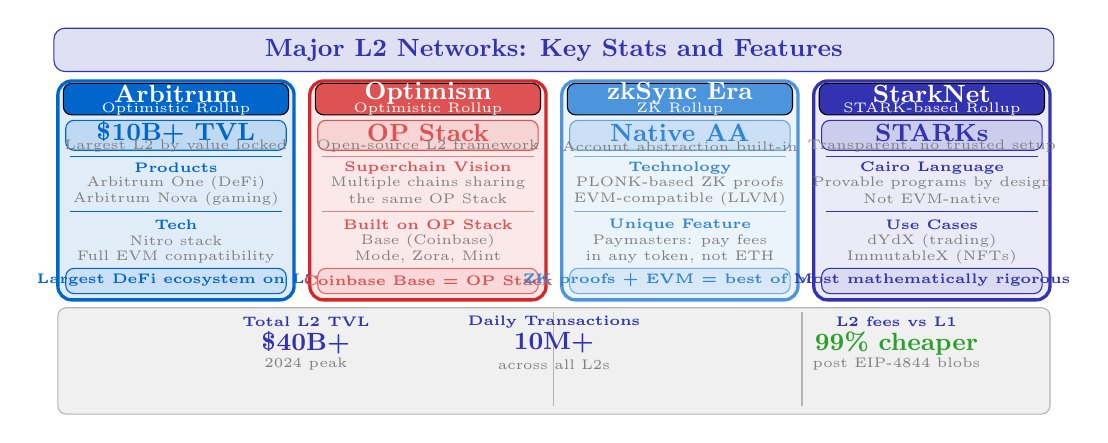
\begin{tikzpicture}
  % Header bar
  \draw[fill=mlpurple!15, draw=mlpurple, rounded corners=4pt] (0.0,4.5) rectangle (12.7,5.05);
  \node[font=\small\bfseries, mlpurple, align=center] at (6.35,4.77) {Major L2 Networks: Key Stats and Features};

  % --- Panel 1: Arbitrum ---
  \draw[fill=mlblue!12, draw=mlblue, very thick, rounded corners=5pt] (0.05,1.6) rectangle (3.05,4.38);
  % Header
  \draw[fill=mlblue, rounded corners=3pt] (0.12,3.95) rectangle (2.98,4.35);
  \node[font=\small\bfseries, white, align=center] at (1.55,4.22) {Arbitrum};
  \node[font=\tiny, white, align=center] at (1.55,4.02) {Optimistic Rollup};
  % Key stat
  \draw[fill=mlblue!25, draw=mlblue, rounded corners=3pt] (0.15,3.5) rectangle (2.95,3.88);
  \node[font=\small\bfseries, mlblue, align=center] at (1.55,3.72) {\$10B+ TVL};
  \node[font=\tiny, mlgray, align=center] at (1.55,3.55) {Largest L2 by value locked};
  % Feature lines
  \draw[mlblue, thin] (0.2,3.42) -- (2.9,3.42);
  \node[font=\tiny\bfseries, mlblue, align=center] at (1.55,3.28) {Products};
  \node[font=\tiny, mlgray, align=center] at (1.55,3.08) {Arbitrum One (DeFi)};
  \node[font=\tiny, mlgray, align=center] at (1.55,2.88) {Arbitrum Nova (gaming)};
  \draw[mlblue, thin] (0.2,2.72) -- (2.9,2.72);
  \node[font=\tiny\bfseries, mlblue, align=center] at (1.55,2.55) {Tech};
  \node[font=\tiny, mlgray, align=center] at (1.55,2.35) {Nitro stack};
  \node[font=\tiny, mlgray, align=center] at (1.55,2.15) {Full EVM compatibility};
  \draw[fill=mlblue!20, draw=mlblue, rounded corners=3pt] (0.15,1.68) rectangle (2.95,2.0);
  \node[font=\tiny\bfseries, mlblue, align=center] at (1.55,1.85) {Largest DeFi ecosystem on L2};

  % --- Panel 2: Optimism ---
  \draw[fill=mlred!10, draw=mlred, very thick, rounded corners=5pt] (3.25,1.6) rectangle (6.25,4.38);
  % Header
  \draw[fill=mlred!80, rounded corners=3pt] (3.32,3.95) rectangle (6.18,4.35);
  \node[font=\small\bfseries, white, align=center] at (4.75,4.22) {Optimism};
  \node[font=\tiny, white, align=center] at (4.75,4.02) {Optimistic Rollup};
  % Key stat
  \draw[fill=mlred!20, draw=mlred!80, rounded corners=3pt] (3.35,3.5) rectangle (6.15,3.88);
  \node[font=\small\bfseries, mlred!80, align=center] at (4.75,3.72) {OP Stack};
  \node[font=\tiny, mlgray, align=center] at (4.75,3.55) {Open-source L2 framework};
  % Feature lines
  \draw[mlred!60, thin] (3.4,3.42) -- (6.1,3.42);
  \node[font=\tiny\bfseries, mlred!80, align=center] at (4.75,3.28) {Superchain Vision};
  \node[font=\tiny, mlgray, align=center] at (4.75,3.08) {Multiple chains sharing};
  \node[font=\tiny, mlgray, align=center] at (4.75,2.88) {the same OP Stack};
  \draw[mlred!60, thin] (3.4,2.72) -- (6.1,2.72);
  \node[font=\tiny\bfseries, mlred!80, align=center] at (4.75,2.55) {Built on OP Stack};
  \node[font=\tiny, mlgray, align=center] at (4.75,2.35) {Base (Coinbase)};
  \node[font=\tiny, mlgray, align=center] at (4.75,2.15) {Mode, Zora, Mint};
  \draw[fill=mlred!18, draw=mlred!70, rounded corners=3pt] (3.35,1.68) rectangle (6.15,2.0);
  \node[font=\tiny\bfseries, mlred!80, align=center] at (4.75,1.85) {Coinbase Base = OP Stack};

  % --- Panel 3: zkSync Era ---
  \draw[fill=mlblue!8, draw=mlblue!70, very thick, rounded corners=5pt] (6.45,1.6) rectangle (9.45,4.38);
  % Header
  \draw[fill=mlblue!70, rounded corners=3pt] (6.52,3.95) rectangle (9.38,4.35);
  \node[font=\small\bfseries, white, align=center] at (7.95,4.22) {zkSync Era};
  \node[font=\tiny, white, align=center] at (7.95,4.02) {ZK Rollup};
  % Key stat
  \draw[fill=mlblue!20, draw=mlblue!60, rounded corners=3pt] (6.55,3.5) rectangle (9.35,3.88);
  \node[font=\small\bfseries, mlblue!80, align=center] at (7.95,3.72) {Native AA};
  \node[font=\tiny, mlgray, align=center] at (7.95,3.55) {Account abstraction built-in};
  % Feature lines
  \draw[mlblue!50, thin] (6.6,3.42) -- (9.3,3.42);
  \node[font=\tiny\bfseries, mlblue!80, align=center] at (7.95,3.28) {Technology};
  \node[font=\tiny, mlgray, align=center] at (7.95,3.08) {PLONK-based ZK proofs};
  \node[font=\tiny, mlgray, align=center] at (7.95,2.88) {EVM-compatible (LLVM)};
  \draw[mlblue!50, thin] (6.6,2.72) -- (9.3,2.72);
  \node[font=\tiny\bfseries, mlblue!80, align=center] at (7.95,2.55) {Unique Feature};
  \node[font=\tiny, mlgray, align=center] at (7.95,2.35) {Paymasters: pay fees};
  \node[font=\tiny, mlgray, align=center] at (7.95,2.15) {in any token, not ETH};
  \draw[fill=mlblue!15, draw=mlblue!55, rounded corners=3pt] (6.55,1.68) rectangle (9.35,2.0);
  \node[font=\tiny\bfseries, mlblue!80, align=center] at (7.95,1.85) {ZK proofs + EVM = best of both};

  % --- Panel 4: StarkNet ---
  \draw[fill=mlpurple!10, draw=mlpurple, very thick, rounded corners=5pt] (9.65,1.6) rectangle (12.65,4.38);
  % Header
  \draw[fill=mlpurple, rounded corners=3pt] (9.72,3.95) rectangle (12.58,4.35);
  \node[font=\small\bfseries, white, align=center] at (11.15,4.22) {StarkNet};
  \node[font=\tiny, white, align=center] at (11.15,4.02) {STARK-based Rollup};
  % Key stat
  \draw[fill=mlpurple!25, draw=mlpurple, rounded corners=3pt] (9.75,3.5) rectangle (12.55,3.88);
  \node[font=\small\bfseries, mlpurple, align=center] at (11.15,3.72) {STARKs};
  \node[font=\tiny, mlgray, align=center] at (11.15,3.55) {Transparent, no trusted setup};
  % Feature lines
  \draw[mlpurple, thin] (9.8,3.42) -- (12.5,3.42);
  \node[font=\tiny\bfseries, mlpurple, align=center] at (11.15,3.28) {Cairo Language};
  \node[font=\tiny, mlgray, align=center] at (11.15,3.08) {Provable programs by design};
  \node[font=\tiny, mlgray, align=center] at (11.15,2.88) {Not EVM-native};
  \draw[mlpurple, thin] (9.8,2.72) -- (12.5,2.72);
  \node[font=\tiny\bfseries, mlpurple, align=center] at (11.15,2.55) {Use Cases};
  \node[font=\tiny, mlgray, align=center] at (11.15,2.35) {dYdX (trading)};
  \node[font=\tiny, mlgray, align=center] at (11.15,2.15) {ImmutableX (NFTs)};
  \draw[fill=mlpurple!18, draw=mlpurple, rounded corners=3pt] (9.75,1.68) rectangle (12.55,2.0);
  \node[font=\tiny\bfseries, mlpurple, align=center] at (11.15,1.85) {Most mathematically rigorous};

  % Bottom stats bar
  \draw[fill=lightgray, draw=midgray, rounded corners=3pt] (0.05,0.15) rectangle (12.65,1.5);
  \node[font=\tiny\bfseries, mlpurple, align=center] at (3.2,1.32) {Total L2 TVL};
  \node[font=\small\bfseries, mlpurple, align=center] at (3.2,1.05) {\$40B+};
  \node[font=\tiny, mlgray, align=center] at (3.2,0.78) {2024 peak};
  \draw[midgray, thin] (6.35,0.25) -- (6.35,1.45);
  \node[font=\tiny\bfseries, mlpurple, align=center] at (6.35,1.32) {Daily Transactions};
  \node[font=\small\bfseries, mlpurple, align=center] at (6.35,1.05) {10M+};
  \node[font=\tiny, mlgray, align=center] at (6.35,0.78) {across all L2s};
  \draw[midgray, thin] (9.5,0.25) -- (9.5,1.45);
  \node[font=\tiny\bfseries, mlpurple, align=center] at (10.7,1.32) {L2 fees vs L1};
  \node[font=\small\bfseries, mlgreen, align=center] at (10.7,1.05) {99\% cheaper};
  \node[font=\tiny, mlgray, align=center] at (10.7,0.78) {post EIP-4844 blobs};
\end{tikzpicture}

\bottomnote{The L2 ecosystem has matured rapidly. Arbitrum and Optimism dominate by TVL; zkSync and StarkNet lead in ZK technology. Total L2 activity now regularly exceeds Ethereum L1 transaction volume.}
\end{frame}

% Frame 10: Key Takeaways
\begin{frame}{Key Takeaways}
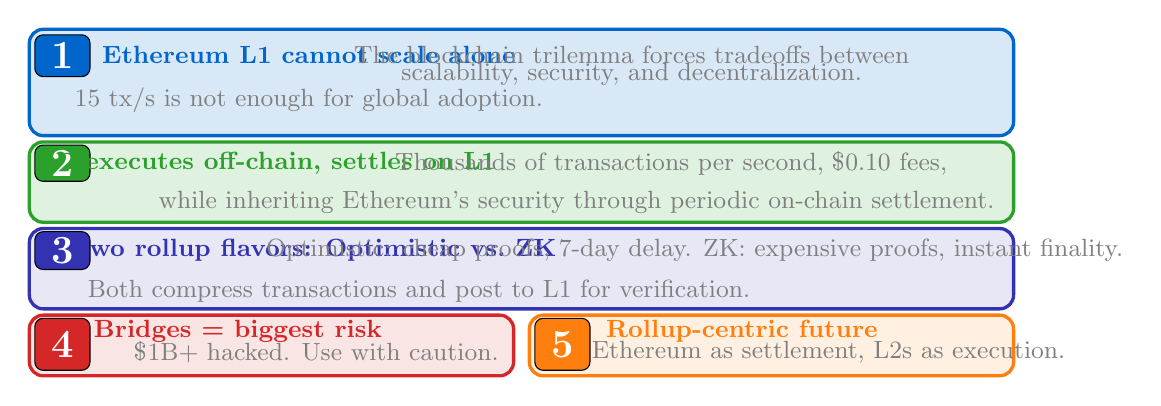
\begin{tikzpicture}
  % Box 1
  \draw[fill=mlblue!15, draw=mlblue, very thick, rounded corners=5pt] (0.05,3.2) rectangle (12.55,4.55);
  \draw[fill=mlblue, rounded corners=3pt] (0.12,3.95) rectangle (0.82,4.48);
  \node[font=\Large\bfseries, white, align=center] at (0.47,4.22) {1};
  \node[font=\small\bfseries, mlblue, align=center] at (3.6,4.22) {Ethereum L1 cannot scale alone};
  \node[font=\small, mlgray, align=center] at (7.7,4.22) {The blockchain trilemma forces tradeoffs between};
  \node[font=\small, mlgray, align=center] at (7.7,3.98) {scalability, security, and decentralization.};
  \node[font=\small, mlgray, align=center] at (3.6,3.65) {15 tx/s is not enough for global adoption.};

  % Box 2
  \draw[fill=mlgreen!15, draw=mlgreen, very thick, rounded corners=5pt] (0.05,2.1) rectangle (12.55,3.12);
  \draw[fill=mlgreen, rounded corners=3pt] (0.12,2.62) rectangle (0.82,3.08);
  \node[font=\Large\bfseries, white, align=center] at (0.47,2.85) {2};
  \node[font=\small\bfseries, mlgreen, align=center] at (3.1,2.85) {L2 executes off-chain, settles on L1};
  \node[font=\small, mlgray, align=center] at (8.2,2.85) {Thousands of transactions per second, \$0.10 fees,};
  \node[font=\small, mlgray, align=center] at (7.0,2.35) {while inheriting Ethereum's security through periodic on-chain settlement.};

  % Box 3
  \draw[fill=mlpurple!12, draw=mlpurple, very thick, rounded corners=5pt] (0.05,1.0) rectangle (12.55,2.02);
  \draw[fill=mlpurple, rounded corners=3pt] (0.12,1.5) rectangle (0.82,1.98);
  \node[font=\Large\bfseries, white, align=center] at (0.47,1.74) {3};
  \node[font=\small\bfseries, mlpurple, align=center] at (3.65,1.74) {Two rollup flavors: Optimistic vs.\ ZK};
  \node[font=\small, mlgray, align=center] at (8.5,1.74) {Optimistic: cheap proofs, 7-day delay. ZK: expensive proofs, instant finality.};
  \node[font=\small, mlgray, align=center] at (5.0,1.22) {Both compress transactions and post to L1 for verification.};

  % Box 4
  \draw[fill=mlred!12, draw=mlred, very thick, rounded corners=5pt] (0.05,0.15) rectangle (6.2,0.92);
  \draw[fill=mlred, rounded corners=3pt] (0.12,0.22) rectangle (0.82,0.88);
  \node[font=\Large\bfseries, white, align=center] at (0.47,0.55) {4};
  \node[font=\small\bfseries, mlred, align=center] at (2.7,0.72) {Bridges = biggest risk};
  \node[font=\small, mlgray, align=center] at (3.7,0.45) {\$1B+ hacked. Use with caution.};

  % Box 5
  \draw[fill=mlorange!12, draw=mlorange, very thick, rounded corners=5pt] (6.4,0.15) rectangle (12.55,0.92);
  \draw[fill=mlorange, rounded corners=3pt] (6.47,0.22) rectangle (7.17,0.88);
  \node[font=\Large\bfseries, white, align=center] at (6.82,0.55) {5};
  \node[font=\small\bfseries, mlorange, align=center] at (9.1,0.72) {Rollup-centric future};
  \node[font=\small, mlgray, align=center] at (10.2,0.45) {Ethereum as settlement, L2s as execution.};
\end{tikzpicture}

\vspace{0.1cm}
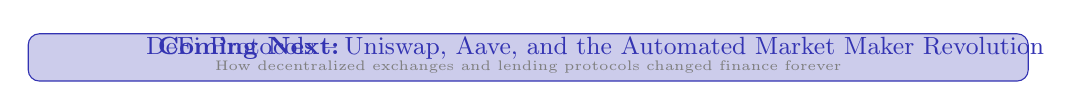
\begin{tikzpicture}
  \draw[fill=mllavender3, draw=mlpurple, rounded corners=4pt] (0,0) rectangle (12.7,0.6);
  \node[font=\small\bfseries, mlpurple] at (2.8,0.42) {Coming Next:};
  \node[font=\small, mlpurple] at (7.2,0.42) {DeFi Protocols -- Uniswap, Aave, and the Automated Market Maker Revolution};
  \node[font=\tiny, mlgray] at (6.35,0.18) {How decentralized exchanges and lending protocols changed finance forever};
\end{tikzpicture}

\bottomnote{Layer 2 is not a workaround -- it is the roadmap. Ethereum's future is a settlement layer secured by cryptographic proofs, with diverse L2 networks handling execution at scale.}
\end{frame}

\end{document}
